So suppose $\abs{\psi(0,x)}^2$ is Gaussian with expetation 0 and standard deviation $\frac{1}{\sqrt{2}}\delta$:
$$\braket{x}{\psi(0)} =\psi(x,0) = \frac{e^{\frac{x^2}{2\Delta}}}{(\pi \Delta^2)^{\frac{1}{4}}}$$
The average position of particle is then
$$\mel{\psi(0)}{X}{\psi(0)}  = \int_{-\infty}^{\infty}  \dd{x'} \braket{\psi(0)}{x'} \mel{x'}{x}{\psi(0)} = \int_{-\infty}^{\infty}  \dd{x'} \psi(x',0) \braket{x'}{\psi(0)} = \int_{-\infty}^{\infty}  \dd{x'} \abs{\psi(x',0)}^2 x' = 0 $$
Now
$$\mel{\psi(0)}{\Delta X^2}{\psi(0)} = \frac{\Delta^2}{2}$$
where
$$\Delta X = X -\mel{\psi(0)}{X}{\psi(0)}$$
Now we want to calculate momentum:
$$\mel{\psi(0)}{P}{\psi(0)} = \int \dd{x'} \psi(x', 0)^*  \mel{x'}{P}{\psi(0)} = \int \dd{x'} \psi(x', 0)^* \qty( -i\hbar \pdv{x'} \psi(x',0)) = 0  $$
and its variance
$$\mel{\psi(0)}{\Delta P^2}{\psi(0)} = \frac{\hbar^2}{2\Delta^2}$$
To find probability density of momentum of particle, we need to find $\abs{\braket{p}{\psi(0)}}^2$:
$$\braket{p}{\psi(0)} = \int \dd{x} \braket{p}{x} \braket{x}{\psi(0)} = \int \dd{x} \frac{1}{\sqrt{2\pi}\hbar} e^{-ipx} \psi(x,0) $$

If we choose
$$\psi(x,0) = \frac{e^{\frac{x^2}{2\Delta}}}{(\pi \Delta^2)^{\frac{1}{4}}} e^{-\frac{ipx}{\hbar}}$$
$$\expval{x} = \mel{\psi(0)}{x}{\psi(0)} = 0$$
$$\expval{\Delta x} = \mel{\psi(0)}{\Delta x}{\psi(0)} = \frac{\Delta}{\sqrt{2}}$$
and
$$\expval{P} = p_0$$
$$\expval{\Delta P} = \frac{\hbar}{\sqrt{2}\Delta}$$

Now we want to find $\psi(x,t)$, for that we search for $c$:
$$c(p) = \frac{1}{\sqrt{2\pi} \hbar} \int_{-\infty}^\infty \dd{x} e^{-\frac{ipx}{\hbar}} \psi(x,0) = \dots = \frac{1}{\sqrt{\hbar}} \frac{e^{-\frac{(p-p_0)^2\Delta^2}{2\hbar^2}}}{\qty(\frac{\pi}{\Delta^2})^{\frac{1}{4}}} $$
Thus
$$\psi(x,t) = \frac{1}{\sqrt{2\pi \hbar}} \int_{-\infty}^\infty \dd{p} c(p) e^{i\qty(px-\frac{p_0}{m}t)\frac{1}{\hbar}} =\frac{1}{\pi^{\frac{1}{4}}\qty(\Delta + \frac{i\hbar t}{m\Delta})^{\frac{1}{2}}} \exp[{-\frac{\qty(x-\frac{p_0}{m}t)^{2}}{2\Delta^2\qty(1 + \frac{i\hbar t}{m\Delta^2})}}] e^{i\frac{p_0}{\hbar} \qty(x-\frac{p_0}{m}t)} $$
And thus probability density
$$P(x,t) = \abs{\psi(x,t) }^2 = \frac{1}{\sqrt{\pi \qty(\Delta^2 + \frac{\hbar^2 t^2}{m^2\Delta^2})}} \exp[{-\frac{\qty(x-\frac{p_0}{m}t)^2}{\Delta^2 + \frac{\hbar^2 t^2}{m^2\Delta^2}}}] $$
Thus
$$\expval{x} = \frac{p_0}{m}t$$
$$\expval{p} = p_0$$
$$\Delta x = \frac{\Delta}{\sqrt{2}} \sqrt{1 + \frac{\hbar^2 t^2}{m^2\Delta^4}}$$
$$\Delta p = \frac{\hbar}{\sqrt{2}\Delta}$$

For small $t$,
$$\Delta x \approx \frac{\Delta}{\sqrt{2}} \qty( 1 + \frac{\hbar^2 t^2}{m^2\Delta^4} + \order{t^4})$$
For large $t$
$$\Delta x \approx  \frac{\hbar t}{\sqrt{2} m\Delta}$$

\paragraph{Substitute numbers}
Suppose $m=1g$ and $\Delta =10^{-13} cm$ - size of proton.

For large $t$
$$\Delta x = 10^{-14}\frac{cm}{s} \cdot t$$
Thus a time we'll need to wait $10^{13}$ seconds until uncertainty becomes an order of $10^{-1} cm$.

\paragraph{Substitute numbers}
For electron, $m\approx 9 \cdot 10^{-28}$ with same $\Delta$. We get
$$\Delta x \approx 10^{13}\frac{cm}{s} \cdot t$$
\subsection{Almost constant potential}
\paragraph{Constant potential}
For $V=V_0$ lets solve
$$H\ket{E} = E\ket{E}$$
$$\mel{x}{\frac{p^2}{2m}+V_0}{E} = E\psi_E(x)$$
, where $\psi_E(x) = \braket{x}{E}$.
$$\qty(-\frac{\hbar}{2m}\pdv[2]{x} + V_0) \psi_E(x) = E\psi_E(x)$$
$$-\frac{\hbar}{2m}\pdv[2]{x}  \psi_E(x) = (E-V_0)\psi_E(x) = \tilde{E} \psi_E(x)$$
Thus we get same solution, just with $\tilde{E}$ instead of $E$:
$$\psi_E(x) = c_{\pm}e^{\pm\frac{\sqrt{2m\tilde{E}}x}{\hbar}}$$
for $\tilde{E}>0$.
\paragraph{Step potential}
$$V = \begin{cases}
0&x<0\\V_0 & x>0
\end{cases}$$
\subparagraph{$E<V_0$}
For $x<0$ we get solution with $0$ potential:
$$\psi_E(x) = c_+ e^{\frac{ipx}{\hbar}} + c_- e^{-\frac{ipx}{\hbar}}$$
For $x>0$:
$$\psi_E(x) = c_+ e^{\frac{\sqrt{2m(V_0-E)}x }{\hbar}} + c_- e^{\frac{\sqrt{2m(V_0-E)}x }{\hbar}}$$
Here, the solutions don't diverge, since $x\in(0, \infty)$, thus only $c_+ = 0$.

Denote $\kappa = \sqrt{2m(V_0-E)}$
$$\psi(x) = \begin{cases}
A_+ e^{\frac{ipx}{\hbar}} + B_- e^{-\frac{ipx}{\hbar}} & x<0\\
C e^{\frac{\sqrt{2m(V_0-E)}x }{\hbar}} & x> 0
\end{cases}$$
Now we want $\psi_E$ be twice differentiable:
$$\begin{cases}
A+B=C\\
\frac{ip}{\hbar} (A-B) = \frac{\kappa}{\hbar} C
\end{cases}$$
From that we can find $A(C)$ and $B(C)$, and $C$, as usual can be find from $\braket{E}{E'}=\delta(E-E') \Rightarrow \int_{-\infty}^\infty \abs{\psi_E(x)}^2 \dd{x} = 1$.

\subparagraph{$E>V_0$}
$$\Psi_E(x) = \begin{cases}
Ae^{-\frac{ipx}{\hbar}}+Be^{\frac{ipx}{\hbar}}& x<0\\
Ce^{-\frac{i\tilde{p}x}{\hbar}}+De^{\frac{i\tilde{p}x}{\hbar}}& x<0\\
\end{cases}$$
From differentiability we get two bound conditions: we can get rid of two constants, say, $A$ and $B$. Thus, for each eigenvalue there are two solutions: with $C=0$ and $D=0$.

\paragraph{Example}
Suppose we have some particle in negative half of plane with momentum in positive direction. Since Hamiltonian is hermitian, we can rewrite $\psi_0$ in eigenbasis.
$$\psi_0(x) = \sum_i c_i \psi_{E_i} (x)$$
\begin{center}
	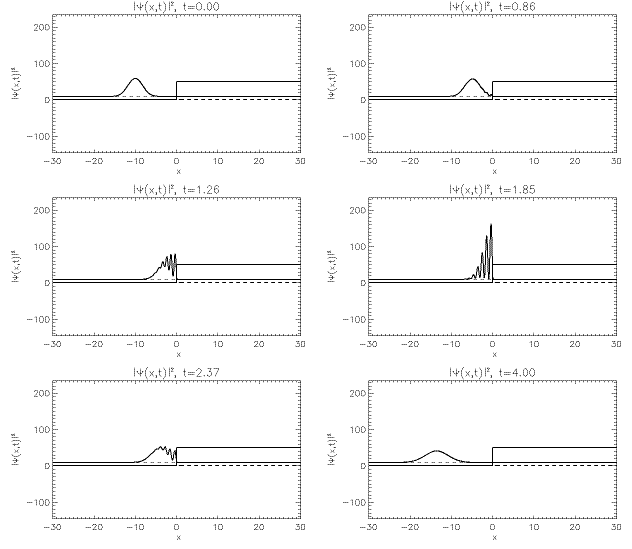
\includegraphics[width=0.5\linewidth]{./lect8/pic1.png}
\end{center}
\subsubsection{Potential well}
\begin{center}
	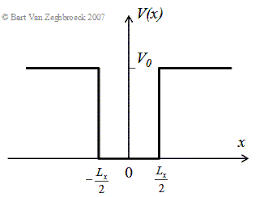
\includegraphics[width=0.4\linewidth]{./lect8/pic2.png}
\end{center}
$$V = \begin{cases}
-V_0 & 0<x<l\\
0 & \text{otherwise}
\end{cases}$$
Thus
$$\psi_E(x) = \begin{cases}
Ae^{\frac{\kappa x}{\hbar}}& x<0\\
Ce^{\frac{ipx}{\hbar}} +De^{\frac{-ipx}{\hbar}} & 0<x<L\\
Be^{\frac{\kappa x}{\hbar}}& x>L\\
\end{cases}$$
From differentiability we can get rid of 2 constants in 0, and from 2 more in $l$. Thus in general, there is no solution, the only case is for specific values of $E$.